% ----------------------------------------------------------
% Histórico dos tipos de aplicações
% ----------------------------------------------------------
\chapter[Fundamentos]{Fundamentos}
%\addcontentsline{toc}{chapter}{Histórico}
% ----------------------------------------------------------

Neste capítulo serão apresentadas algumas das pricipais soluções utilizadas para a construção de aplicações. Ele mostra um pouco da evolução nas arquiteturas de aplicações, partindo de modelos simples como o IPC, passando pelas arquiteturas de duas e três camadas, até as arquiteturas distribuídas, como o SOA. 


\section{IPC - Comunicação entre processos}\label{sec:ipc}

Nem sempre um programa sequencial é a melhor solução para um determinado problema. Muitas vezes, as implementações são estruturadas na forma de várias tarefas inter-dependentes que cooperam entre si para atingir os objetivos da aplicação \cite{sistemas-op-mazierro}. Diversos sistemas operacionais fornecem mecanismos para viabilizar a comunicação e o compartilhamento de dados entre aplicações. Coletivamente, as atividades habilitadas por estes mecanismos são chamadas de Interprocess Communications (IPC) \cite{microsoft-ipc}.

IPC consiste em mecanismos que garantem a comunicação entre processos concorrentes e os acessos aos recursos compartilhados. Algumas formas de IPC facilitam a divisão de trabalho entre diversos processos especialistas, enquanto outras facilitam esta divisão entre computadores dentro de uma rede.

Normalmente, os aplicativos que fazem parte de uma comunicação através de IPC são categorizados como clientes ou servidores. Um cliente é um aplicativo ou um processo que solicita um serviço de alguma outra aplicação ou processo. Por outro lado um servidor é um aplicativo ou um processo que responde a uma solicitação de cliente. Muitas aplicações agem como um cliente e servidor, dependendo da situação \cite{microsoft-ipc}.

A figura \ref{fig:how-communication-works} mostra como ocorre a comunicação entre processos (P1 P2, P3 e P4). Esta troca de informação pode acontecer de duas maneiras: em duas etapas, ou de forma direta. A comunicação em duas etapas, ilustrada na figura através de flechas, envolve um processo coordenador, que pode ser um interpretador em Python por exemplo, utilizado para dar início ao \textit{workflow}. Na figura, a comunicação em duas etapas ocorre entre os processos P1 e P2, fazendo uso de um processo coordenador. A comunicação direta é ilustrada na figura ligada por linhas pontilhadas e não necessita de intermediação de nenhum processo. Esta maneira de comunicação pode ser executada através de diversas formas, entre elas: \textit{Pipes}, \textit{Shared Memory}, \textit{Mapped Memory} e arquivos compartilhados.

\begin{figure}
    \centering
    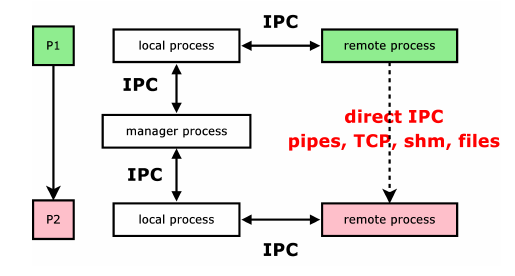
\includegraphics[width=0.7\textwidth]{figuras/ipc.png}
    \caption{Características dos mecanismos de comunicação }
    \legend{Fonte: \citeonline{sistemas-op-mazierro}}
    \label{fig:how-communication-works}
\end{figure}

\section{Cliente/Servidor}\label{sec:clientserver}

Também conhecido como arquitetura de duas camadas, o modelo cliente/servidor consiste em uma arquitetura em que a camada de apresentação se encontra no cliente e a camada de dados encontra-se no servidor. Esta separação se opõe ao modelo centralizado amplamente utilizado até seu surgimento.

O processamento dos dados é dividido em duas partes distintas. Uma parte é a requerente de dados (cliente), e a outra parte é a provedora dos dados (servidor). O cliente envia durante sua execução uma ou mais solicitações ao servidor para realizar alguma tarefa específica. É de responsabilidade do cliente tanto apresentar as informações para o usuário, quanto executar as regras de negócio necessárias à aplicação. O servidor é responsável por armazenar os dados e fornecer um meio para que o cliente os consulte \cite{two-tier}.

Desde a década de 1990, fornecedores de \textit{software} desenvolvem e trazem ao mercado muitas ferramentas para simplificar o desenvolvimento de aplicativos para a arquitetura cliente/servidor de duas camadas. Algumas das mais conhecidas são: Microsoft Visual Basic, Delphi da Borland e PowerBuilder da Sybase. Estas ferramentas combinadas com uma comunidade ativa de desenvolvedores, fizeram da abordagem de duas camadas cliente/servidor uma solução econômica para criação diversos tipos de sistemas.

Desde então, aplicações \textit{desktop} comunicando-se com o servidor de banco de dados se tornaram um caso de uso normal. A maior parte da lógica de negócios foi incorporada dentro da aplicação \textit{desktop}. Portanto, esse estilo de clientes na aquitetura de duas camadas também foi chamado de \textit{fat clients}.

A figura \ref{fig:two-tier} ilustra como a arquitetura em duas camadas funciona, mantendo uma comunicação direta entre cliente e servidor, sem intermediários entre as duas pontas. Visto que neste modelo as regras de negócio estão presentes na camada de aplicação, ele é frequentemente aplicado em ambientes homogêneos. Como a camada de banco de dados e a camada de aplicação estão fisicamente próximos, este modelo também oferece um bom desempenho para as aplicações.

\begin{figure}[htbp]
    \centering
    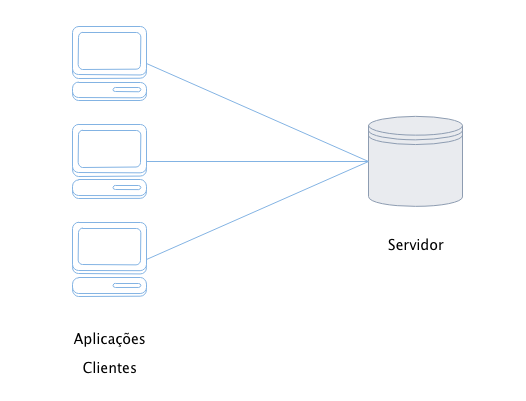
\includegraphics[width=0.7\textwidth]{figuras/client-server.png}
    \caption{Comunicação em duas camadas}
    \label{fig:two-tier}
\end{figure}

Por outro lado, o modelo cliente servidor em duas cadamas possui grandes desafios de escalabilidade. Quando múltiplos usúarios executam requisições simultâneas, a aplicação perde muito desempenho, dado ao fato que cada cliente precisa de conexão de banco de dados separadas e processamento de CPU exclusivo para executar as requisições. Entretando, um dos maiores problemas na arquitetura em duas camadas ocorre quando há mudanças na estrutura do banco de dados. A maioria das aplicações cliente dependem da estrutura do banco de dados, o que impede qualquer remodelagem deste, criando um problema de estruturas legadas, e muitas vezes subutilizadas \cite{two-tier-differences}.

O modelo de aplicações cliente/servidor foi substituido pelo modelo de três camadas, muito mais eficiente, e que fornece uma maneira de dividir as funcionalidades envolvidas na manutenção e apresentação de uma aplicação.

\section{Aplicações Monolíticas}\label{sec:monolitico}

Conforme \citeonline{monolithic-definition} explica, uma aplicação monolítica é construída como uma única unidade de \textit{software}. Estas aplicações são construídas em três camadas: um banco de dados (que consiste em tabelas geralmente em um sistema de gerenciamento de banco de dados), uma interface de usuário do lado do cliente (consistindo de páginas executando em um navegador ou aplicativos móveis) e um lado do servidor de aplicação. Esta aplicação do lado do servidor trata as requisições HTTP, executa as regras de negócio, recupera e atualiza registros do banco de dados e constrói as respostas para serem enviadas às aplicações clientes. 

Estas camadas representam uma aplicação monolítica - um único executável lógico, e para fazer alterações no sistema, é necessário criar e implantar uma versão atualizada do aplicativo do lado do servidor. Uma aplicação monolítica é autônoma e independente de outras aplicações. A filosofia do projeto consiste em um aplicativo que não é responsável apenas por uma determinada tarefa, mas que também pode executar todos os passos necessários para completar uma determinada função, como é mostrado na figura \ref{fig:three-tier}.

\begin{figure}[htbp]
    \centering
    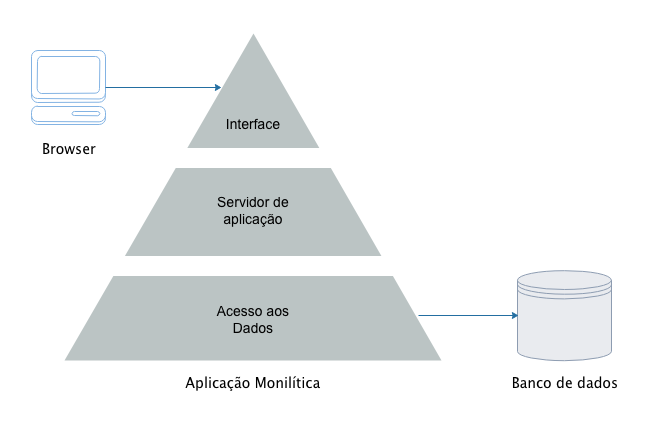
\includegraphics[width=0.7\textwidth]{figuras/monolithic-3-tier.png}
    \caption{Aplicação monolítica clássica em 3 camadas}
    \label{fig:three-tier}
\end{figure}

\citeonline{monolithic-extinction} afirma que o modelo monolítico é uma maneira natural para a evolução de uma aplicação. A maioria das aplicações começam com um único objetivo, ou um pequeno número de objetivos relacionados. Ao longo do tempo, novas funcionalidades são adicionados ao aplicativo para suportar as necessidades do negócio. Entretando, as aplicações monolíticas apresentam algumas desvantagens, sendo algumas delas: 

\begin{enumerate}[label=\alph*)]
    \item Um único ponto de falha pode comprometer o funcionamento correto de todos os módulos do sistema.
    \item Baixa estalabilidade dado a necessidade de copiar toda a \textit{stack} \footnote{Conjunto de ferramentas que formam uma solução de software} para o escalonamento horizontal.
    \item Base de código volumosa, a medida que a aplicação cresce, uma vez que toda a regra de negócio se encontra em uma só base.
    \item É necessária muita comunicação para que várias equipes de desenvolvedores trabalhem em paralelo. Esta sobrecarga diminui o ritmo de desenvolvimento.
\end{enumerate}

Contudo, com a popularização dos \textit{frameworks} Javascript como Angular e Backbone, houve um movimento de desacoplamento da camada de visualização nas aplicações monolíticas. Foram criadas então as chamadas aplicações \textit{frontend}, responsáveis pela camada de apresentação, e sendo executadas em dispositivos móveis como \textit{smartphones} e \textit{tables} ou nos \textit{browsers desktop}. 

Esse movimento criou um modelo monolítico de duas camadas, ilustrado na figura \ref{fig:two-tier-monolithic}. A remoção da interdependência entre as camadas de interface e o servidor de aplicação facilitou o escalonamento e a escalabilidade de cada uma das partes. Esta separação de conceitos foi o primeiro passo em direção a uma arquitetura mais orientada a serviços.

\begin{figure}[htbp]
    \centering
    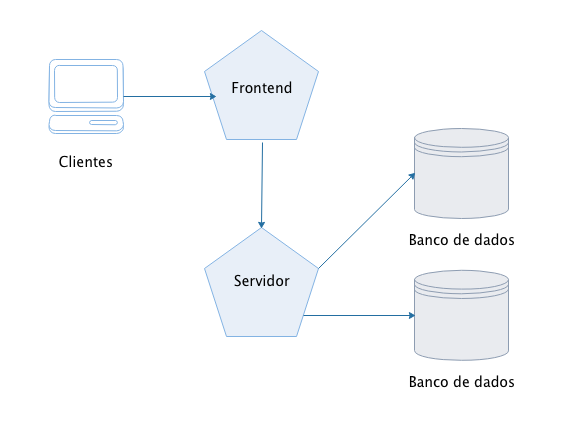
\includegraphics[width=0.7\textwidth]{figuras/monolithic-2-tier.png}
    \caption{Modelo monolítico de duas camadas}
    \label{fig:two-tier-monolithic}
\end{figure}

\section{SOA - Service Oriented Architecture}\label{sec:soa}

\citeonline{soa-cbdi} define SOA como políticas, práticas e \textit{frameworks} que permitem que rotinas de aplicações sejam fornecidas e consumidas como conjuntos de serviços publicados em uma granularidade relevante para o consumidor do serviço. Estes serviços podem ser invocados, publicados e descobertos, e são abstraídos da implementação usando uma única forma de interface baseada em padrões.

Além de criar e expor serviços, \citeonline{soa-tech-target} assinala que a SOA tem a capacidade de aproveitar tais serviços de forma recursiva em aplicações (conhecidos como aplicativos compostos). Para isto, ela pode atuar como uma arquitetura orquestradora de serviços, ou expor cada um deles individualmente. Um aspecto importante da SOA é a separação da interface de serviço (o que) da sua implementação (como). Esses serviços são consumidos por clientes que não estão preocupados com a forma como esses eles irão executar suas solicitações

 A SOA permite a reutilização de ativos existentes, em que novos serviços podem ser criados a partir de uma infraestrutura de sistemas de TI existente. Em outras palavras, ela permite que as empresas reutilizem aplicativos existentes e possibilita a interoperabilidade entre aplicações e tecnologias heterogêneas. Ela fornece um nível de flexibilidade que não era possível antes, no sentido de que:

 \begin{enumerate}[label=\alph*)]
    \item Os serviços são componentes de \textit{software} com interfaces bem definidas e independentes da implementação.
    \item Os serviços são autônomos (executam tarefas predeterminadas) e vagamente acoplados (para independência);
    \item Serviços compostos podem ser construídos a partir de agregados de outros serviços;
\end{enumerate}

Isso significa que a SOA é uma abordagem alinhada com o negócio, em que os aplicativos dependem dos serviços disponíveis para facilitar os processos de negócios. Um serviço é um componente de \textit{software} reutilizável e autônomo, fornecido por um provedor de serviços e consumido pelos solicitantes. A SOA cria uma visão de flexibilidade de TI que facilita a agilidade do negócio. Sua implementação envolve principalmente componentes de aplicativos corporativos e/ou em desenvolvimento que usam serviços, disponibilizando aplicativos como serviços para outras aplicações \cite{soa-book}.

\citeonline{soa-tech-target} acrescenta que em um ambiente SOA típico, existe um provedor de serviços e um consumidor de serviços. Para que isso funcione, também é necessário um mecanismo para que eles possam se comunicar uns com os outros, como é ilustrado na figura \ref{fig:soa}. A W3C \footnote{World Wide Web Consortium} definiu um padrão aberto para que \textit{web services} possam implementar a SOA e habilitar a comunicação entre o provedor e o consumidor através de um protocolo baseado em XML: o \textit{Simple Object Access Protocol} (SOAP). Outros padrões também são usados ou foram criados para realizar a comunicações entre os serviçoes SOA. Alguns exemplos são o \textit{REpresentation State Transfer} (REST), que utiliza tanto XML quando JSON para transportar os dados entre os serviços, ou mais recentemente o GraphQL, utilizando um modelo declaraivo de comunicação entre o cliente e o servidor, também baseado em JSON.

\begin{figure}[htbp]
    \centering
    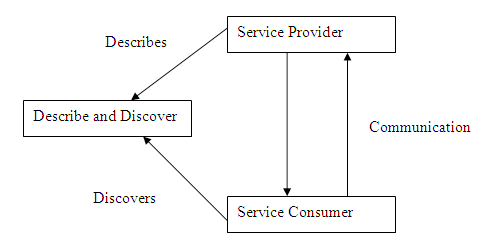
\includegraphics[width=0.7\textwidth]{figuras/soa.png}
    \caption{Service Oriented Architecture}
    \label{fig:soa}
\end{figure}

Em geral, há uma confusão entre o relacionamento entre SOA e \textit{web services}. \citeonline{soa-webservice} faz uma distinção entre estes dois conceitos do seguinte modo: "Web services tratam-se de especificações de tecnologias, enquanto o SOA é um princípio de \textit{design} de \textit{software}. Notavelmente, Web services são um padrão de definição de interface adequado para a SOA e é neste ponto onde eles se conectam". Portanto, SOA é um padrão de arquitetura, enquanto os \textit{Web services} são serviços implementados usando um conjunto de padrões. \textit{Web service} é uma das maneiras em que é possível implementar a SOA, e por isso compartilha dos mesmo benefícios já citados relacionados a SOA.

As arquiteturas para construção de aplicações evoluiram de modelos centralizadas em direção a modelos mais distribuídos, com objetivo de dividir melhor a responsabilidade de cada um de seus componentes. 